\documentclass[10pt,draftclsnofoot,onecolumn]{IEEEtran}
\hyphenation{op-tical net-works semi-conduc-tor}

\usepackage[margin=.75in]{geometry}
\usepackage{courier}
\usepackage{ifthen}
\usepackage{setspace}
\usepackage{listings}
\usepackage[usenames, dvipsnames]{color}
\usepackage{tabularx}
\usepackage[strict]{chngpage}
\usepackage{cite}
\usepackage{graphicx}
\usepackage{acronym}
\usepackage{color}
\usepackage{makeidx}

\makeindex

\acrodef{OSU}[OSU]{Oregon State University}
\acrodef{AIAA}[AIAA]{American Institute of Aeronautics and Astronautics}
\acrodef{AGL}[AGL]{Above Ground Level}

\lstset {
	language=C,
	basicstyle=\ttfamily,
	keywordstyle=\color{blue}\ttfamily,
	stringstyle=\color{red}\ttfamily,
	commentstyle=\color{OliveGreen}\ttfamily,
	morecomment=[l][\color{magenta}]{\#}
	showstringspaces=false,
	showspaces=false,
	frame=single,
	captionpos=b
}

\newcommand{\commandline}[2][\empty] {
	\begin{quote}
		\texttt{#2}
		\ifthenelse{\equal{#1}{\empty}}{}{\begin{quote}#1\end{quote}}
	\end{quote}
}

\newcommand{\sigline}[1][\empty] {
	\vspace{1in}
	\hrule width0.5\textwidth
	\vspace{1mm}
	\noindent #1	
}

\begin{document}
	\singlespace
	
	\title{\vspace{2in}Problem Statement}
	
	\author {
		Anisimova, Natasha
		\and
		Lee, Terrance
		\and
		Morgan, Albert
	}
	
	\markboth{CS Capstone 2016-2017}{Groundstation}
	
	\pagestyle{empty}
	\vspace*{2in}
	\begin{center}
		\huge
		Groundstation: Requirements\\
		\normalsize
		\vspace{5mm}
		\textbf{
			Team \#25\\
			High-Altitude Rocketry Challenge\\
		}
		\vspace{1mm}
		Natasha Anisimova\\
		Terrance Lee\\
		Albert Morgan
	\end{center}
	
	\vspace{5mm}
	
	\begin{center}
		\textbf{Abstract}
	\end{center}
	
	%\begin{adjustwidth}{0.75in}{0.75in}
	
	The \textit{Groundstation} software will collect telemetry from a rocket while it is in flight and graphically display the telemetry in real-time.
	Collecting the telemetry in real-time will reduce the chances of a failure-to-recover by allowing the ground team to track the rocket during its flight.
	The graphical display will make the telemetry instantly understandable without time-consuming analysis.
	This document will detail the specific requirements of the Groundstation software.

	
	%\end{adjustwidth}
	
	\newpage
	
	\tableofcontents
	\newpage
	
	\pagestyle{headings}


	\section{Introduction}
	
	\subsection{Purpose}
	This document will specify the requirements for the Groundstation (GS) software.
	It is intended for use by the OSU High-Altitude Rocketry Team.
	
	\subsection{Scope}
	GS will gather telemetry from a rocket during flight.
	While the telemetry is being gathered, it will be logged and displayed graphically in real-time.
	This software will provide the following benefits to the users:
	\begin{enumerate}
		\item Real-time data will allow the rocket's location to be tracked during flight.
		Allowing this data to be accessed before recovery will aid in the recovery itself.
		\item The graphical display will make the data easy to interpret.
		\item Logging will allow the data to be analyzed at a later date.
		\item Altitude data will give evidence of whether the objective of one hundred thousand feet was met.
	\end{enumerate}	
			
	\subsection{Definitions}
	
	\begin{itemize}
		\index{Accuracy}
		\item \textbf{Accuracy:} The absence of errors in the telemetry GS receives, logs, and displays.
		\index{Binary data}
		\item \textbf{Binary data:} Telemetry that represents one of two states, for example, ``stage 2 activated'' and
		``stage 2 not activated.''
		\index{Corruption}
		\item \textbf{Corruption:} The process by which data is altered or made unreadable.
		\index{Crash}
		\item \textbf{Crash:} A software crash; the event in which a piece of software ceases operation unexpectedly.
		\index{Groundstation}
		\index{GS}
		\item \textbf{GS:} Groundstation, the name of our software.
		\index{Graphical display}
		\item \textbf{Graphical display:} Data that is displayed using a visualization.
		\index{Live}
		\item \textbf{Live:} Updated in real-time.
		\index{Page}
		\item \textbf{Page:} A web page that users of GS may connect to in order to view the telemetry.
		%\index{Lean angle}
		%\item \textbf{Lean angle:} The angle relative to the vertical that the rocket is currently traveling.
		\index{Non-volatile storage}
		\index{Storage}
		\item \textbf{Non-volatile storage:} Storage that will not be erased when the system is powered down.
		For example, a hard drive or flash storage.
		\index{Raspberry Pi}
		\item \textbf{Raspberry Pi:} A small, inexpensive computing platform.		
		\index{Real-time}
		\item \textbf{Real-time:} Each telemetry datum received from the rocket must be processed and
		displayed in under one second.
		\index{Redundant sensors}
		\item \textbf{Redundant sensors:} Two or more sensors that provide the same type of data.
		\index{Reliability}
		\item \textbf{Reliability:} In the event of a software crash, the Groundstation software should automatically
		start and begin all normal functions in under five seconds.
		\index{Robustness}
		\item \textbf{Robustness:} In the event that GS receives data that is garbled or otherwise does adhere
		to the protocol, it must continue to receive and display data and not break the real-time requirement.
		\index{Storage}
		\item \textbf{Storage:} A device where data is logged.		
		\index{Telemetry}
		\item \textbf{Telemetry:} Data received from the rocket while the rocket is in flight.
		\index{Telemetry packet}
		\index{Packet}
		\item \textbf{Telemetry packet:} The rocket will send a telemetry update once per second. Each one of these updates is a ``telemetry packet.''
		\index{Vizualation}
		\item \textbf{Visualization:} Information or data, transformed into an visual context.
	\end{itemize}	
	
	\subsection{Overview}
	The rest of this document contains specific requirements about the functionality and constraints of GS. This includes
	the needs of the entire rocketry team, the physical constraints of the system, and the limitations of the launch site.
	
	\textit{Overall description} gives a high-level view of the functions of the software and describes any constraints.
	\textit{Specific requirements} gives a detailed list of requirements that were proposed by the OSU High-Altitude
	Rocketry Team and describes specific requirements and constraints.
		
	
	\section{Overall description}
	\subsection{Product perspective}
	GS will receive data from a serial interface, via hardware and a protocol provided by the avionics team.
	Due to the launch site not having any connection to the Internet or mobile service, GS will not interact with
	any outside systems. 
	Additionally, GS will provide a software interface that allows users to view the telemetry,
	graphically, in real-time.
	\subsection{Product functions}
	GS provides two major functions while the rocket is in flight:
	
	\begin{enumerate}
		\index{Logging}
		\item Telemetry logging to non-volatile storage.
		\item Display of real-time graphical data. 
	\end{enumerate}
	
	\subsection{User characteristics}
	\index{Users}
	The users of this software will be limited to engineering students and advisors who are part of the OSU High-Altitude
	Rocketry Team.
	These users will be expected to be familiar with the software and the rocket launch.
	Because the software team works closely with the rest of the rocketry team on regular basis,
	any training necessary will be conducted in-person.
	
	\subsection{Constraints}
	\index{Constraints}
	\begin{itemize}
		\item Because of the remote nature of launch sites, the software must operate without an Internet connection.
		\item The software must be as reliable as is reasonably possible, and additional features must not compromise the reliability.
		\item Groundstation will receive telemetry via a protocol that is TBD by the avionics team.
	\end{itemize}
	\subsection{Assumptions and dependencies}
	\index{Raspberry Pi}
	Groundstation will run on a Raspberry Pi with no Internet connectivity.
	
	\subsection{Apportioning of requirements}
	
	\begin{figure}
		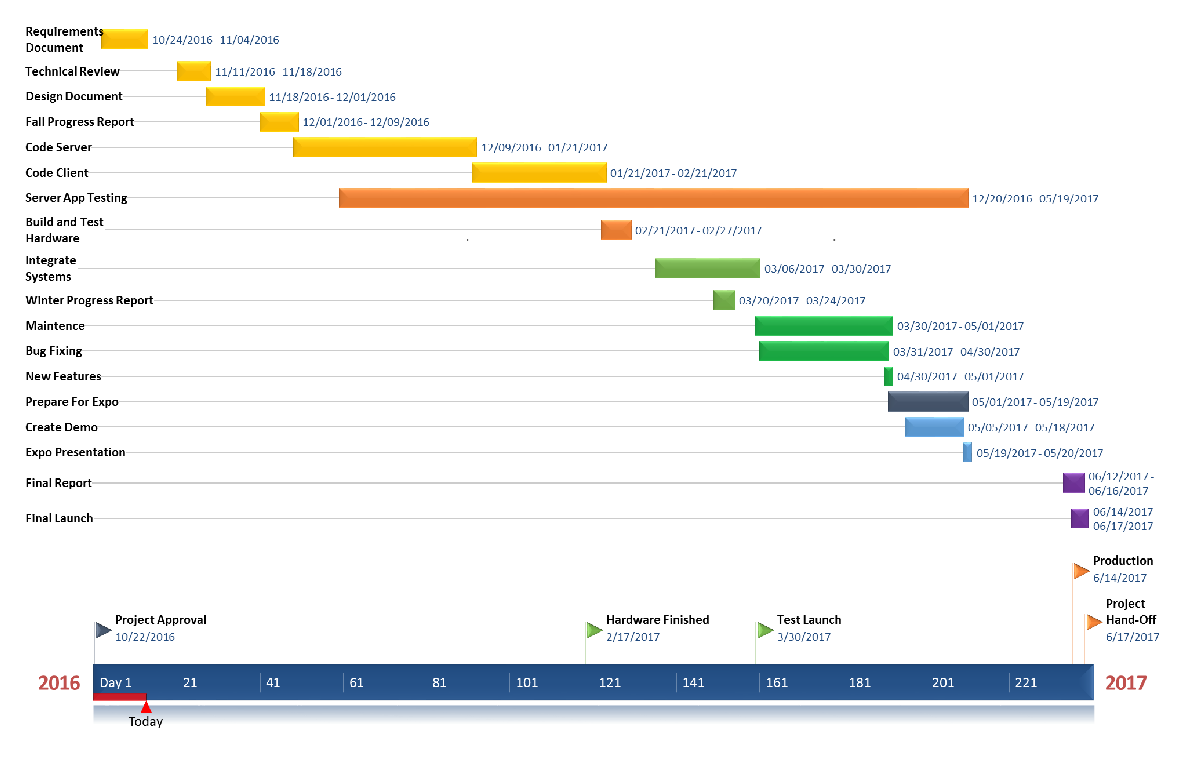
\includegraphics[width=\linewidth]{ganttchart.eps}
		\caption{A Gantt chart outlining the work to be done over the next nine months.}
		\label{fig:gantt}
	\end{figure}
	
	Figure \ref{fig:gantt} shows a gantt chart outlining our schedule from now until the first test rocket launch.
	Although the final rocket launch is on 23 June, all core systems of GS should be finished by the test launch in mid-May.
		
	\section{Specific requirements}
	
	\subsection{External interface requirements}
	\subsubsection{User interfaces}
	Users will interact with GS by connecting via a web browser. The Raspberry Pi and other associated hardware,
	to be provided by the avionics team,
	will broadcast a wireless network that users will connect to and access GS through a web browser.
	From this page, users will be able to access the graphical display of the telemetry.
	
	GS will support Google Chrome version 54 and higher. Users running other browsers or older versions of Chrome
	may not be able to connect to GS.
	\subsubsection{Hardware interfaces}
	GS will run on a Raspberry Pi broadcasting a wireless network. Users will connect to GS with their personal computers
	via the wireless network.

	Data is received from a serial interface using a protocol that will be determined by the avionics team.
	
	\subsection{System Features}
	
	The stimulus for all specific requirements is receiving a new piece of telemetry. The specific responses will be described here.


% I've commented out the non-essential requirements here.
% These are poorly defined "stretch" goals, and don't belong in this document.
		
	\begin{itemize}
		\item GS will collect data from a serial interface using a yet-to-be-determined protocol designed by the High-Altitude Rocketry Team's avionics section.
		\item GS will log all telemetry in real-time to non-volatile storage so that it can be analyzed
		after the launch.
		The data from the serial port will be written to directly to non-volatile storage in order to limit
		the possibility of corruption.
		\item The graphical display shall be updated in real-time.
		\item Users will connect to GS and be able to view a visualzation of the telemetry in real-time.
		\item GS will support a live line graph visualization for altitude data.
		\item GS will have the ability to show the most recently recorded latitude and longitude in a numerical format.
	\end{itemize}
	
	\subsection{Performance requirements}
	
	\begin{itemize}
		\item When a new telemetry packet is received, GS will log the telemetry and update all visualizations in under one second.
		\item GS will support a minimum of 20 concurrent users.
	\end{itemize}


	\subsection{Design constraints}
	\index{Design contraints}
	\index{Contraints}
	\index{Raspberry Pi}
	GS will run on a Raspberry Pi 3 model B, which has a 1.2 GHz quad-core 64-bit ARM Cortex-A53 processor
	with 1 GB of SDRAM memory.

	\subsection{Software system attributes}

	\subsubsection{Reliability}
	\index{Reliability}
	In the event that GS crashes, it should automatically restart and continue
	operation in under five seconds.

	\subsubsection{Robustness}
	\index{Robustness}
	If GS receives corrupted or otherwise incorrectly formatted telemetry, it should not crash.
	Additionally, the users should not be able to crash GS from the web interface.

	\subsubsection{Accuracy}
	\index{Accuracy}
	GS should not introduce any errors in the telemetry it recieves.
	Data should be logged and displayed with 100\% accuracy.

\printindex

% Signatures% Signatures% Signatures% Signatures% Signatures
\begin{minipage}{\textwidth}	
	\sigline{Nancy Squires}
	\sigline{Natasha Anisimova}
	\sigline{Terrance Lee}
	\sigline{Albert Morgan}	
\end{minipage}


\end{document}


